\subsection{Scheduler}
The central scheduler operates in this section regarding communication with the background of our project. In fact, it is responsible for informing the interface process about the pairs $(client, motorcycle)$ that need to be moved. It writes this information into a shared memory segment obtained through the \textbf{shmget()} function and sends a signal to the UI using the \textbf{kill()} function. The UI will then read the information from the shared memory segment and use it to simultaneously move both the motorcycle and the client it carries. The information written includes:
\begin{enumerate}
    \item the client's process ID (pid)
    \item the motorcycle's process ID (pid)
    \item the starting and destination points of the client
\end{enumerate}
The UI will then use this data to carry out the movement.

%After we have recovered the user's interface Pid, we will use it to get the scheduler's PId. This is the command to launch this :\\

%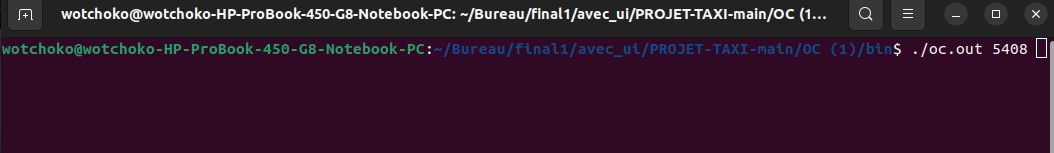
\includegraphics[width=1.0\textwidth]{Sections/Images/oc-out.png}\\

%And this is the result of this command :\\

%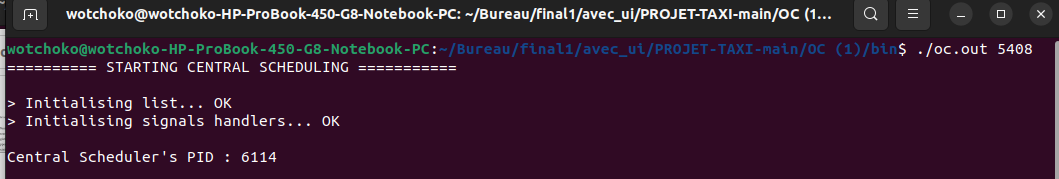
\includegraphics[width=1.0\textwidth]{Sections/Images/oc_pid.png}\\
